%
% Clases de módulo de AHR.
% Análisis y diseño de programa tokenizador, reporte técnico.
%
% Proyecto Lovelace.
%

\subsubsection{Clases de AHR}

AHR utiliza la interfaz \acrshort{gl:cdv} para poder interactuar con la base de
datos y realizar el proceso de detokenización, pues es un algoritmo
irreversible. Hace uso también de algunas utilidades como potencias y
el cálculo del dígito verificador mediante el algoritmo de Luhn desfasado.
Utiliza también la clase del registro al momento de agregar un nuevo token
a la base de datos y la clase de \textit{Arreglo de dígitos} para implementar
los métodos de \textit{tokenizar} y \textit{detokenizar} definidos por la
interfaz \textit{Algoritmo tokenizador irreversible}.

Finalmente, se utiliza la clase AES para realizar el cifrado por bloque; esta
clase es una interfaz y permite utilizar el cifrado de AES por hardware si
el procesador tiene las instrucciones necesarias. En caso de no tenerlo,
cifra mediante las funciones de CryptoPP.

El diagrama de clases de AHR se encuentra en la figura~\ref{clases_ahr}.
\begin{sidewaysfigure}
  \begin{center}
    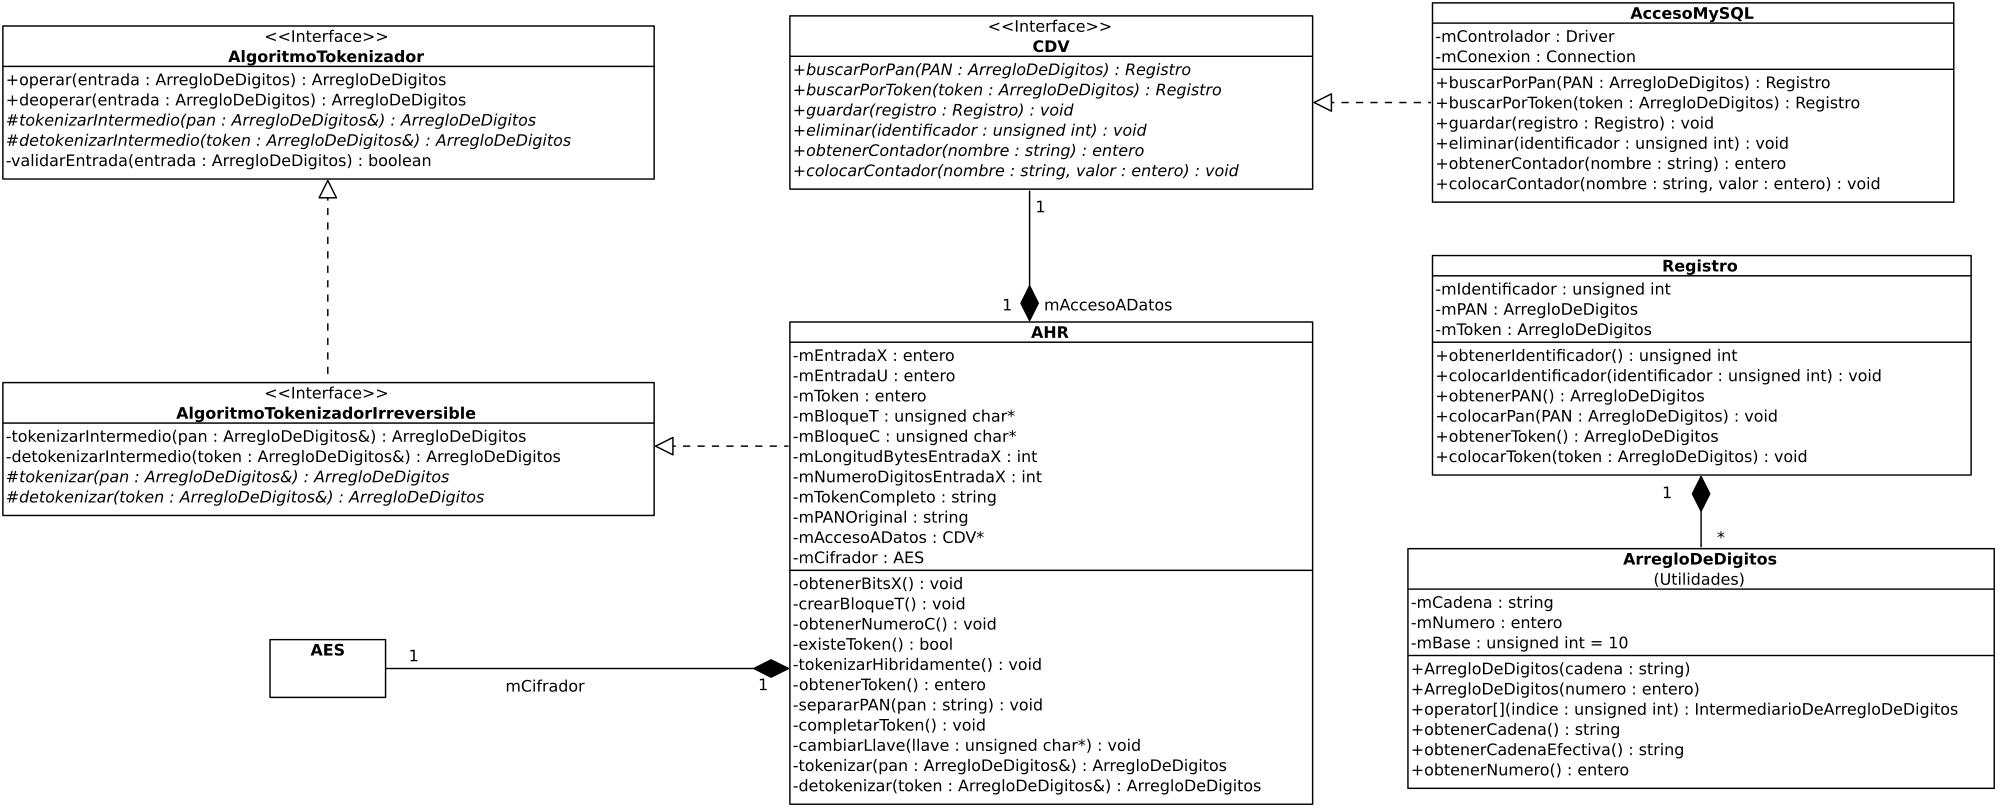
\includegraphics[width=1.0\linewidth]{diagramas/ahr.png}
    \caption{Diagrama de clases de módulo de AHR.}
    \label{clases_ahr}
  \end{center}
\end{sidewaysfigure}
